
\providecommand{\myrootdir}{..}
\documentclass[\myrootdir/main.tex]{subfiles}

\begin{document}

\chapter{Information Extraction Techniques}
\label{models}
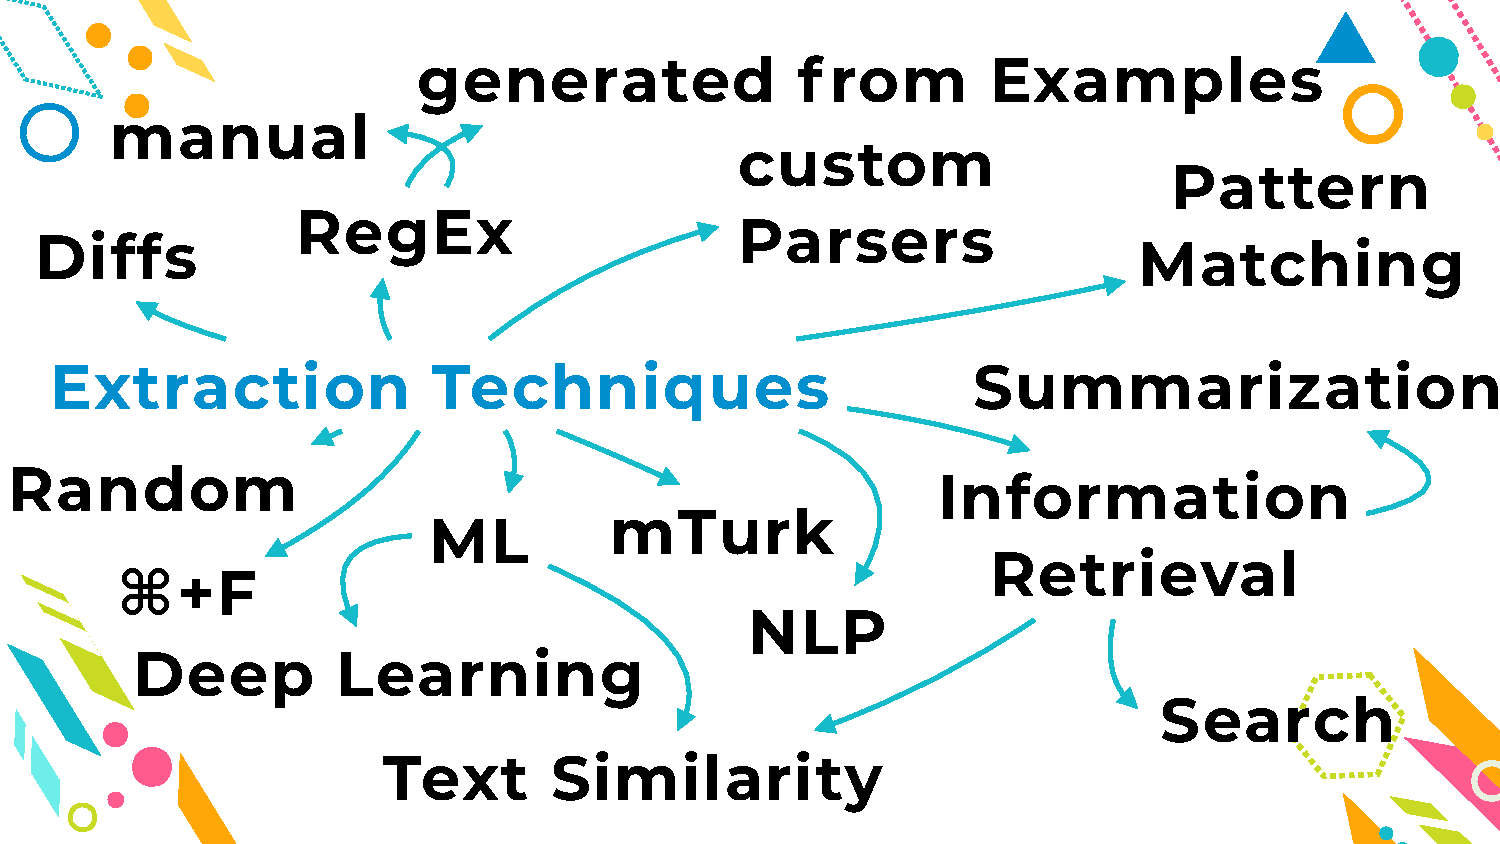
\includegraphics[page=1, width=\textwidth, trim={0.5cm 0.5cm 0.5cm 0.5cm}, clip]{img/RetreatSeptemberSlides.pdf}
Many different information extraction techniques ... this section describes the concepitonal / theoretical results of our thesis ... 
We create a model to characterize BLIE techniques so we can discuss their similarities and differences more clearly. 
Additionally we present a complimentary model for IE tasks, to describe use cases for BLIE techniques in a structured way.
From our analysis of build logs we share our notion of the extractable information within a build log.

\section{Characteristics of a Buildlog}
various tools writing in there, each own internal syntax, no common formatting agreements across tools, Travis Output additional newlines / coloring

\subsection{Comparison to Runtime Logs}
\todo{or did we do that in related work enough?}

\section{Our Model for Information Extraction Techniques}
\includegraphics[page=3, width=\textwidth, trim={0.5cm 0.5cm 0.5cm 0.5cm}, clip]{img/flow-of-research.pdf}
\plan{model = making a picture with boxes to visualize what we are talking about}
A build log information extraction technique (BLIE technique) consumes a build log (text file) and produces a certain output (text). \todo{make picture, output can be contained in log or not, can be continuous substring or selected lines etc.}.
\begin{itemize}
  \item{Target}{Extractable Information} each extraction technique \todo{instantiation!} targets a specific information
  \item{Setup Overhead}{Time}
  \item{Performance}{Performance} split into learning performance
\end{itemize}

Example instantiations of this task later in this chapter, namely for the three techniques we are comparing: PROSE program synthesis, IR text similarity, and simple keyword search. \todo{ref?}

\section{Our Model for Information Extraction Tasks}
\includegraphics[page=4, width=\textwidth, trim={0.5cm 0.5cm 0.5cm 0.5cm}, clip]{img/flow-of-research.pdf}
aims to describe an information extraction task of a developer or a researcher.
\begin{itemize}
  \item \todo{describe all classes}
  \item{Setup Overhead}{Time}
  \item{Performance}{Performance} split into learning performance
\end{itemize}
\todo{give 2-3 concrete example instantiations here}

\section{Our Model for Extractable Information in Build Logs}
\includegraphics[page=2, width=\textwidth, trim={0.5cm 0.5cm 0.5cm 0.5cm}, clip]{img/flow-of-research.pdf}
during our inital exploration \& data collection for the Failing Build Log Data Set, wanted to get an impression about the information one would want to extract from a build log
\begin{itemize}
  \item \todo{describe all classes}
  \item{Setup Overhead}{Time}
  \item{Performance}{Performance} split into learning performance
\end{itemize}
\todo{differentiate Travis CI specific things, explain high variability for instantiations}
\todo{give at least one concrete example instantiation, best from a log in the data set, not too long so maybe it goes in the abstract?, picture/graphic with marked parts here?}


\section{PROSE Program Synthesis}
\includegraphics[page=2, width=\textwidth, trim={0.5cm 0.5cm 0.5cm 0.5cm}, clip]{img/RetreatSeptemberSlides.pdf}
\todo{explanation of process, the way our tool does it, instantiate model of extraction technique, probably no additional theoretical stuff really needed here?, describe regex programs}

\section{IR Similarity}
\includegraphics[page=3, width=\textwidth, trim={0.5cm 0.5cm 0.5cm 0.5cm}, clip]{img/RetreatSeptemberSlides.pdf}
\todo{explanation of process, the way our tool does it, instantiate model of extraction technique, probably no additional theoretical stuff really needed here?}

\section{Keyword search}
\includegraphics[page=4, width=\textwidth, trim={0.5cm 0.5cm 0.5cm 0.5cm}, clip]{img/RetreatSeptemberSlides.pdf}
\todo{explanation of process, the way our tool does it, instantiate model of extraction technique, probably no additional theoretical stuff really needed here?}

\section{Further Techniques}
\todo{maybe: instantiate model, or at least partly talk about it}
\todo{diffing, manual regex?, other summarization?, BART? <- we could reference that from related work then}

\end{document}
